%-----------------------------------------------------------------------------
%
%               Template for sigplanconf LaTeX Class
%
% Name:         sigplanconf-template.tex
%
% Purpose:      A template for sigplanconf.cls, which is a LaTeX 2e class
%               file for SIGPLAN conference proceedings.
%
% Guide:        Refer to "Author's Guide to the ACM SIGPLAN Class,"
%               sigplanconf-guide.pdf
%
% Author:       Paul C. Anagnostopoulos
%               Windfall Software
%               978 371-2316
%               paul@windfall.com
%
% Created:      15 February 2005
%
%-----------------------------------------------------------------------------


\documentclass[preprint,10pt]{sigplanconf}

% The following \documentclass options may be useful:
%
% 10pt          To set in 10-point type instead of 9-point.
% 11pt          To set in 11-point type instead of 9-point.
% authoryear    To obtain author/year citation style instead of numeric.

\usepackage{amsmath}

% http://www.texample.net/tikz/examples/tag/graphs/
\usepackage{tikz}
\usetikzlibrary{arrows}
\usepackage{listings}
\usepackage{hyperref}
% "define" Scala
\lstdefinelanguage{scala}{
  morekeywords={abstract,case,catch,class,def,%
    do,else,extends,false,final,finally,%
    for,if,implicit,import,match,mixin,%
    new,null,object,override,package,%
    private,protected,requires,return,sealed,%
    super,this,throw,trait,true,try,%
    type,val,var,while,with,yield},
  otherkeywords={=>,<-,<\%,<:,>:,\#,@},
  sensitive=true,
  morecomment=[l]{//},
  morecomment=[n]{/*}{*/},
  morestring=[b]",
  morestring=[b]',
  morestring=[b]"""
}


\begin{document}

\conferenceinfo{Scala 2013 '13}{July 2nd, Montpellier.} 
\copyrightyear{2013} 
\copyrightdata{[to be supplied]} 

\titlebanner{banner above paper title}        % These are ignored unless
\preprintfooter{short description of paper}   % 'preprint' option specified.

\title{Parsing your trail through the graph} % Graph Traversal Combinators
\subtitle{Applying the Idea of Parser Combinators to Graph Traversals}

\authorinfo{Daniel Kr\"oni}
           {FHNW}
           {daniel.kroeni@fhnw.ch}
%\authorinfo{Name2\and Name3}
%          {Affiliation2/3}
%         {Email2/3}

\maketitle

\begin{abstract}
%1. State the problem
%2. Say why it�s an interesting problem
%3. Say what your solution achieves
%4. Say what follows from your solution

Connected data such as social networks or biological pathways are commonly modeled as graphs and persisted in graph databases. In contrast to relational databases where SQL is the proven standard query language, there is no established counterpart for graph databases.\\
One way to query a graph is by specifying a path pattern which must be matched. We show how a simple functional combinator library provides an elegant mean to express such patterns by applying the idea of parser combinators to graph traversals. Traversers are composed of primitives such as following an edge and familiar grammar constructions such as sequencing, choice and repetition.\\
The result is a traverser combinator library called "trails" which provides an implementation for \href{http://www.neo4j.org/}{neo4j} and for \href{http://blueprints.tinkerpop.com/}{blueprint api}.  
\end{abstract}

\category{CR-number}{subcategory}{third-level}

\terms
term1, term2

\keywords
keyword1, keyword2

\section{Introduction}

Given a property graph consisting of vertices and edges where both kinds of elements may contain properties (key-value pairs). We describe an elegant solution to ...
Graph traversals can be described similar to formal languages - by using grammar constructions such as sequencing, choice and repetition. A popular approach to language recognition in functional programming are parser combinators. In this paper we show how to adapt the idea of parser combinators to the problem of graph traversal specifications.



\section{The type of traversers}
In a first approximation a traverser is a function that takes a graph as input and returns a path as a result.

\begin{lstlisting}[language=scala]
type Traverser = Graph => Path
\end{lstlisting}

There may be more than one path which fits the specification of a traverser - or none at all. We account for that by letting the result be a stream of paths. In the section about laziness we discuss this decision in more depth.

\begin{lstlisting}[language=scala]
type Traverser = Graph => Stream[Path]
\end{lstlisting}

Some traverser start with an empty path, but most of them describe an extension of an existing path which we call prefix. To model this scenario we extend the type of traverser and add the prefix path as a further input parameter.

\begin{lstlisting}[language=scala]
type Traverser = 
  Graph => Path => Stream[Path]
\end{lstlisting}

Finally a traverser might return a specific value besides the paths, for example the value of a property of an element.

\begin{lstlisting}[language=scala]
type Traverser[A] = 
 Graph => Path => Stream[(Path, A)]
\end{lstlisting}

This is the type of a traverser we will use in this paper.


\section{Primitive traversers}
\begin{itemize}
\item Vertex
\item Edge
\item Filter
\end{itemize}

\section{Traverser combinators}
\begin{itemize}
\item Sequence
\item Choice
\item Repetition
\end{itemize}


\section{Lazyness}
In order to avoid excessive paths computation in setup where a traverser pattern fits many paths, 
laziness allows to compute only as many result paths as needed.

\begin{itemize}
\item depth-first is only sensitive order in a lazy environment.
\end{itemize}



\section{Cycles}
We want the traverser to terminate, even if it describes a cyclic path. What is a cycle? In a graph the answer is common wisdom. But what is a cycle in a path? If an edge is traversed for a second time? No! ...

We propose a definition which is relative to the repetition combinator.

\begin{itemize}
\item slice combinator
\end{itemize}

If a repetition combinator yields the same slice a second time, we consider it a cycle.


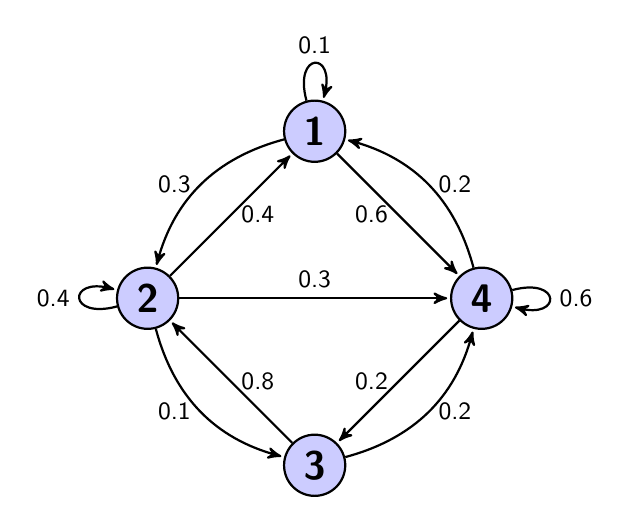
\begin{tikzpicture}[->,>=stealth',shorten >=1pt,auto,node distance=3cm,
  thick,main node/.style={circle,fill=blue!20,draw,font=\sffamily\Large\bfseries}]

  \node[main node] (1) {1};
  \node[main node] (2) [below left of=1] {2};
  \node[main node] (3) [below right of=2] {3};
  \node[main node] (4) [below right of=1] {4};

  \path[every node/.style={font=\sffamily\small}]
    (1) edge node [left] {0.6} (4)
        edge [bend right] node[left] {0.3} (2)
        edge [loop above] node {0.1} (1)
    (2) edge node [right] {0.4} (1)
        edge node {0.3} (4)
        edge [loop left] node {0.4} (2)
        edge [bend right] node[left] {0.1} (3)
    (3) edge node [right] {0.8} (2)
        edge [bend right] node[right] {0.2} (4)
    (4) edge node [left] {0.2} (3)
        edge [loop right] node {0.6} (4)
        edge [bend right] node[right] {0.2} (1);
\end{tikzpicture}

\section{Labels}

\appendix
\section{Appendix Title}

This is the text of the appendix, if you need one.

\acks

Acknowledgments, if needed.

% We recommend abbrvnat bibliography style.

\bibliographystyle{abbrvnat}

% The bibliography should be embedded for final submission.

\begin{thebibliography}{}
\softraggedright

\bibitem[Smith et~al.(2009)Smith, Jones]{smith02}
P. Q. Smith, and X. Y. Jones. ...reference text...

\end{thebibliography}

\end{document}
